% !TeX root = ../main.tex
% !TeX root = ../main.tex
\section{Синтез согласующих цепей и анализ устойчивости}

\subsection{Исследование устойчивости и выбор рабочей точки генератора}

На частоте $f = 4{,}5\text{ ГГц}$ транзистор NE68133 находится в области потенциальной устойчивости ($K \approx 0{,}92 < 1$). В ходе параметрического анализа было установлено, что критерий безусловной устойчивости ($K \ge 1$) за счёт индуктивной обратной связи в цепи эмиттера достигается лишь при чрезмерно больших значениях индуктивности порядка $L_E \approx 24\text{ нГн}$. Однако при этом предельный коэффициент усиления каскада катастрофически деградирует до величины $G_{\max} \approx 0{,}13\text{ дБ}$, что делает усилитель полностью неработоспособным.

В связи с этим в качестве инженерного компромисса выбрано физически реализуемое значение технологической индуктивности выводов $L_E = 1{,}2\text{ нГн}$, при котором сохраняется коэффициент передачи $G = 1{,}71\text{ дБ}$, а устойчивость каскада обеспечивается выбором импеданса источника $\Gamma_S$ вне областей потенциального самовозбуждения.

На рис.~\ref{fig:smith_analysis} представлены результаты анализа на диаграмме Воль\-пер\-та--Сми\-та на частоте $f = 4{,}5\text{ ГГц}$. На рис.~\ref{fig:smith_analysis},~а приведено совместное отображение окружности шума ($NF = 0{,}15\text{ дБ}$), окружности доступного усиления ($G_a = 1{,}2\text{ дБ}$) и годографа входного коэффициента отражения $S_{11}$. На рис.~\ref{fig:smith_analysis},~б приведены окружности устойчивости со стороны источника ($\mathrm{KCS}$) и нагрузки ($\mathrm{KCL}$).

\begin{figure}[H]
    \centering
    \begin{minipage}{0.48\textwidth}
        \centering
        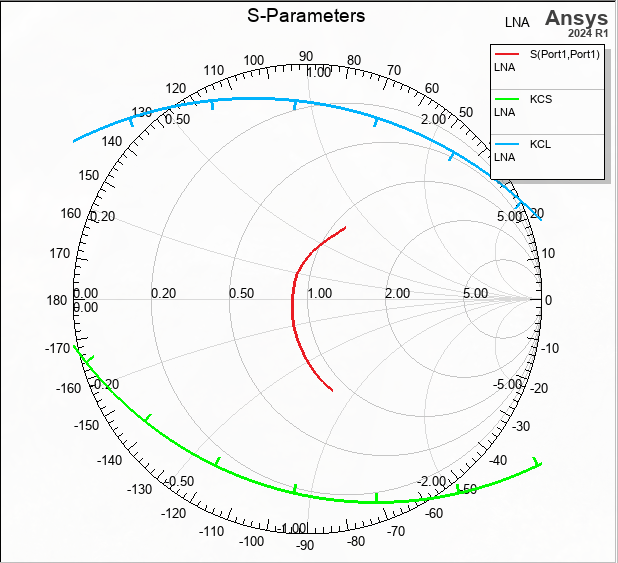
\includegraphics[width=\textwidth]{export_figs/01_smith.png}
        \caption*{а) Окружности $NF$ и $G_a$}
    \end{minipage}\hfill
    \begin{minipage}{0.48\textwidth}
        \centering
        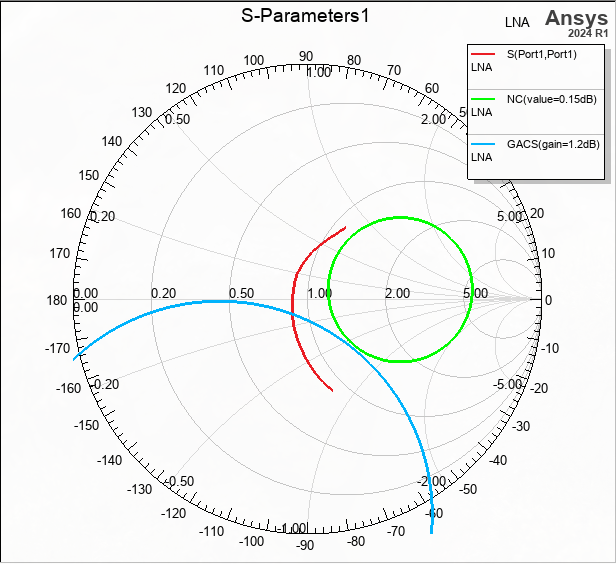
\includegraphics[width=\textwidth]{export_figs/02_smith.png}
        \caption*{б) Окружности устойчивости $\mathrm{KCS}$ и $\mathrm{KCL}$}
    \end{minipage}
    \caption{Анализ транзистора на диаграмме Вольперта--Смита ($f = 4{,}5\text{ ГГц}$, $L_E = 1{,}2\text{ нГн}$)}
    \label{fig:smith_analysis}
\end{figure}

Рабочая точка коэффициента отражения генератора $\Gamma_S$ выбирается в области допустимого шума вблизи центра диаграммы, что обеспечивает баланс между минимальным коэффициентом шума каскада и сохранением устойчивости при приемлемом согласовании по входу.

\subsection{Синтез входной и выходной цепей согласования}

Для согласования стандартных 50-омных трактов источника и нагрузки с оптимальными импедансами транзистора на рабочей частоте $f_0 = 4{,}5\text{ ГГц}$ был выполнен расчёт Г-образных реактивных цепей в среде диаграммы Воль\-пер\-та--Сми\-та (рис.~\ref{fig:smith_mapping}).

\begin{figure}[H]
    \centering
    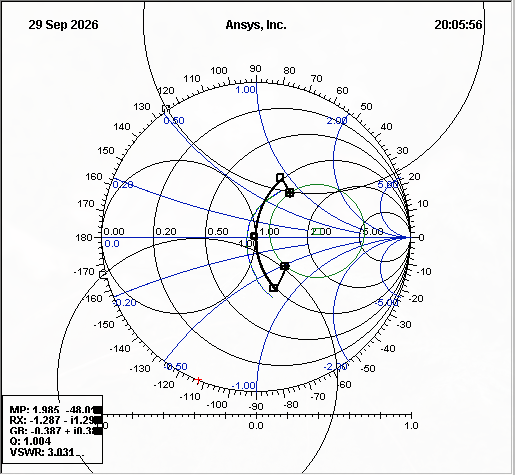
\includegraphics[width=0.68\textwidth]{export_figs/03_smith.png}
    \caption{Траектории трансформации импедансов согласующих цепей на диаграмме Вольперта--Смита}
    \label{fig:smith_mapping}
\end{figure}

Синтез входной согласующей цепи (Input Matching Network) осуществляется с помощью Г-образного звена из двух сосредоточенных реактивных элементов:
\begin{enumerate}
    \item Параллельно включённая индуктивность $L_{\text{вх}} = 8{,}28\text{ nH}$, компенсирующая реактивную составляющую входного импеданса на частоте $4{,}5\text{ ГГц}$;
    \item Последовательно включённый конденсатор $C_{\text{вх}} = 1{,}09\text{ pF}$, обеспечивающий окончательную трансформацию сопротивления источника ($50\text{ Ом}$) в требуемый импеданс генератора $\Gamma_S$, а также выполняющий функцию развязки по постоянному току базы транзистора.
\end{enumerate}

Выходная согласующая цепь (Output Matching Network) также представляет собой Г-образное звено:
\begin{enumerate}
    \item Параллельный конденсатор $C_{\text{вых}} = 104{,}5\text{ fF}$ со стороны коллектора транзистора;
    \item Последовательная индуктивность $L_{\text{вых}} = 1{,}62\text{ nH}$, трансформирующая выходной импеданс каскада к стандартной нагрузке $50\text{ Ом}$.
\end{enumerate}

Сводные значения номиналов элементов приведены в табл.~\ref{tab:matching_elements}.

\begin{table}[H]
\centering
\caption{Номиналы элементов согласующих цепей усилителя ($f_0 = 4{,}5\text{ ГГц}$)}
\label{tab:matching_elements}
\resizebox{\textwidth}{!}{%
\begin{tabular}{|l|c|c|}
\hline
\textbf{Цепь согласования} & \textbf{Параллельный элемент} & \textbf{Последовательный элемент} \\ \hline
Входная цепь (Input Matching)   & $L_{\text{вх}} = 8{,}28\text{ nH}$    & $C_{\text{вх}} = 1{,}09\text{ pF}$   \\ \hline
Выходная цепь (Output Matching) & $C_{\text{вых}} = 104{,}5\text{ fF}$  & $L_{\text{вых}} = 1{,}62\text{ nH}$  \\ \hline
Эмиттерная ОС                   & \multicolumn{2}{c|}{$L_E = 1{,}2\text{ nH}$} \\ \hline
\end{tabular}%
}
\end{table}

\subsection{Моделирование схемы усилителя в Ansys Designer}

Принципиальная схема спроектированного малошумящего усилителя с синтезированными цепями согласования в среде моделирования Ansys Designer представлена на рис.~\ref{fig:schematic}.

\begin{figure}[H]
    \centering
    \includegraphics[width=0.78\textwidth]{01_sch.png}
    \caption{Принципиальная схема LNA в среде Ansys Designer}
    \label{fig:schematic}
\end{figure}

На рис.~\ref{fig:s_parameters} приведены частотные зависимости расчетных $S$-параметров спроектированного усилителя в полосе частот от $0{,}5$ до $5{,}0\text{ ГГц}$.

\begin{figure}[H]
    \centering
    \includegraphics[width=0.82\textwidth]{01_rect.png}
    \caption{Рассчитанные $S$-параметры усилителя в диапазоне частот $0{,}5\dots 5{,}0\text{ ГГц}$}
    \label{fig:s_parameters}
\end{figure}

Анализ полученных характеристик на центральной частоте $f_0 = 4{,}5\text{ ГГц}$ показывает:
\begin{itemize}
    \item \textbf{Коэффициент усиления} $\mathrm{dB}(S_{21}) \approx +2{,}0\text{ дБ}$, что полностью соответствует расчётному значению доступного усиления $G_a$ с учётом стабилизирующей эмиттерной индуктивности $L_E$;
    \item \textbf{Выходное согласование} $\mathrm{dB}(S_{22}) \approx -12{,}5\text{ дБ}$, что удовлетворяет общепринятому инженерному критерию ($\mathrm{dB}(S_{22}) < -10\text{ дБ}$, $\text{КСВН} < 1{,}9$);
    \item \textbf{Входное согласование} $\mathrm{dB}(S_{11}) \approx -9{,}5\dots -10\text{ дБ}$, гарантирующее отсутствие значительных отражений мощности источника;
    \item \textbf{Коэффициент обратной передачи} $\mathrm{dB}(S_{12}) < -6\text{ дБ}$, подтверждающий достаточную развязку каскада.
\end{itemize}

Небольшое уширение полосы согласования и смещение минимума кривой $S_{22}$ в область $3{,}75\dots 4{,}2\text{ ГГц}$ обусловлено влиянием внутренней комплексной обратной связи транзистора через эмиттерную катушку $L_E$, а также дискретностью номиналов сосредоточенных компонентов.
